%======================================================================
\section{Zero-shot transfer in one dimension}
\label{sec:results1d}
%======================================================================

The 1D model is trained at $L=100$ on whole periodic domains of $P=16$
sites ($h=6.25$, sixteen grid points per site) with $c=3$ channels, so
$\dlat=48$ (Appendix~\ref{app:architecture}). We then load the same
weights, unchanged, into models with $P=4,8,32$ and $64$ sites
(Corollary~\ref{cor:transfer}); every parameter is copied with no missing
or unused entries, and nothing is retrained.

%----------------------------------------------------------------------
\subsection{At the trained size}
%----------------------------------------------------------------------

At $L=100$ the model has $\lambda_1=0.094$--$0.098$ and 12 positive
exponents out of 48 from each of three initial conditions, against
$\lambda_1=0.090$ and 12 positive exponents for the PDE, and
$\DKY=22.24\pm0.11$ against $22.49$, $1.1\%$ low. A sibling model with
twice the latent dimension ($P=32$, $\dlat=96$) has 13 positive exponents
out of 96: doubling the coordinates barely changes the number of unstable
directions, so the 48-dimensional latent is not short of capacity.

%----------------------------------------------------------------------
\subsection{Transfer to other domain sizes}
%----------------------------------------------------------------------

Table~\ref{tab:transfer1d} and Fig.~\ref{fig:transfer1d} compare the
transferred model with independent ground truth at every size. From
$L=50$ to $L=400$, a factor of 8 in domain size, the model's $\DKY$ lies
$0.2$--$1.2\%$ below the truth, and the error does not grow as the
domain moves away from the trained size ($0.2\%$ at $L=400$). The model's
density $\DKY/L$ is $0.222$--$0.223$ at every size, against
$0.224$--$0.226$ for the PDE: the model is extensive, as a local model
must be (Remark~\ref{rem:extensive_model}), with a density about $1\%$
below the true one. Each truth is the mean of two or three independent
finite-time runs; their spread ($0.1$--$2\%$) is comparable to the
model's offset at $L=50$ and $L=200$ (Table~\ref{tab:transfer1d}).

\begin{table*}[htbp]
\caption{Zero-shot transfer of the 1D model trained at $L=100$.
$P$: sites; truth from Table~\ref{tab:truth}, mean $\pm$ half-range over
its independent runs. Model: mean $\pm$ half-range over three initial
conditions standardized with the training statistics; $n_+$: number of
positive exponents (range over initial conditions); error: model mean
relative to truth mean.}
\label{tab:transfer1d}
\begin{ruledtabular}
\begin{tabular}{rrrcccrr}
$L$ & $P$ & $\dlat$ & true $\DKY$ & model $\DKY$ & $n_+$ & error & model $\DKY/L$ \\
\hline
\tabinput{tables/tab03_transfer1d}
\end{tabular}
\end{ruledtabular}
\end{table*}

\begin{figure*}[htbp]
\centering
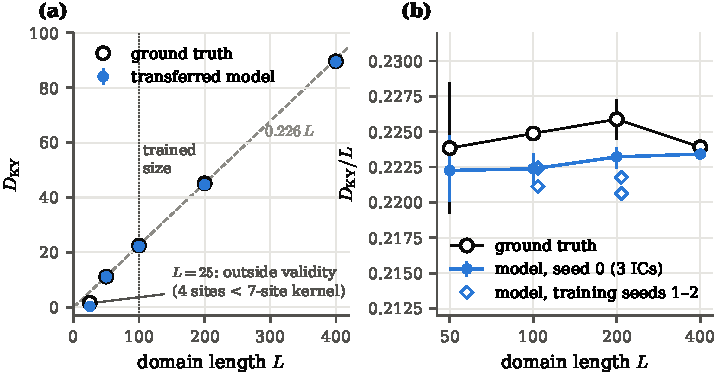
\includegraphics{figures/fig03_1d_transfer.pdf}
\caption{Zero-shot transfer of the 1D KS model trained at $L=100$.
(a) Kaplan--Yorke dimension of the PDE (open circles) and of the
transferred model (filled) against domain length; the dashed line is
$0.226L$. At $L=25$ the transferred lattice has 4 sites, fewer than one
propagator kernel spans, and the size is outside the model's domain of
validity (text). (b) Dimension per unit length for $L\ge50$, including
two independently trained models (diamonds) at $L=100$ and $L=200$; note
the vertical range, $0.2125$--$0.2325$. Bars span three initial
conditions (model) and two or three independent finite-time runs
(truth). The model sits $0.2$--$1.2\%$ below the truth at every size.}
\label{fig:transfer1d}
\end{figure*}

\begin{figure*}[htbp]
\centering
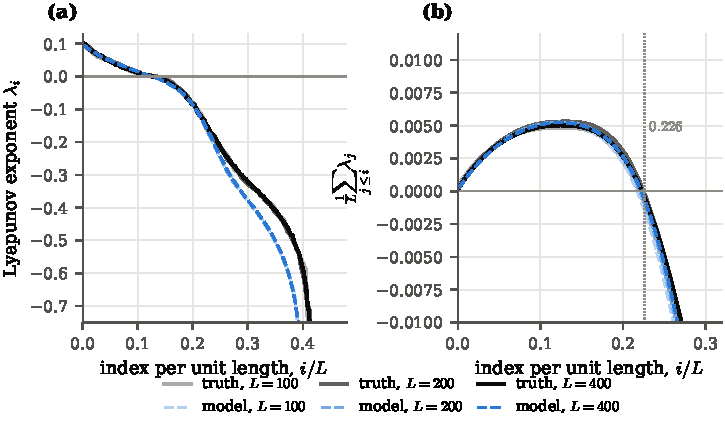
\includegraphics{figures/fig04_1d_spectra.pdf}
\caption{Lyapunov spectra of the transferred 1D model (dashed, blue) and of
the PDE (solid, gray to black) at $L=100$, $200$ and $400$; lighter lines
are smaller domains. (a) Exponents against index per unit length. (b)
Cumulative sum per unit length; it crosses zero at the Kaplan--Yorke
dimension density, marked at $0.226$. Model spectra are averaged
index-wise over three initial conditions.}
\label{fig:spectra1d}
\end{figure*}

\para{Training seeds.} Two further models trained with the same recipe
and different random seeds give $\DKY/L = 0.2224$ and $0.2211$ at $L=100$
and $0.2218$ and $0.2206$ at $L=200$, against $0.2224$ and $0.2232$ for
the first (mean over three initial conditions). The three seeds agree to
within $0.6\%$ at the trained size and $1.2\%$ after transfer, the same
order as one model's spread over initial conditions. The transfer is a
property of the recipe, not of one checkpoint.

\para{Where transfer stops.} At $L=25$ the PDE is at most marginally
chaotic: its leading exponent, $0.0013$ over 1200 time units, is barely
distinguishable from zero, and its $\DKY$ ($1.56$ or $1.82$ depending on
the number of tangent directions) is poorly determined. The transferred
model has 4 sites, fewer than the 7 that one propagator kernel spans, so
its circular convolutions wrap onto themselves
(Appendix~\ref{app:proofs}); it is non-chaotic from two of three initial
conditions and has one positive exponent ($\DKY=1.10$) from the third.
This size is outside the model's domain of validity by construction, and
we do not score it.

\para{Beyond the dimension.} The agreement is not confined to $\DKY$:
the whole positive and near-neutral part of the Lyapunov spectrum,
plotted against $i/L$, collapses onto the truth's at all three sizes,
with a mean difference of $0.002$--$0.003$ per exponent
(Fig.~\ref{fig:spectra1d}). The model departs from the truth only in the
strongly contracting directions beyond $i/L\approx0.22$, where its
exponents are more negative; these do not enter $\DKY$. Free rollouts of
the transferred model stay bounded at every size, and the largest $|u|$
over a rollout is $3.3$--$3.7$ against $3.3$--$3.5$ for the PDE
at $L=100$--$400$. Over 900 time units of free rollout, the decoded
field's energy in each of five wavenumber bands is within about $10\%$ of
the PDE's at all three sizes (Fig.~\ref{fig:rollouts}(a--c)), and the
autoencoder alone reconstructs the field to $0.01\%$ of its variance
(Appendix~\ref{app:tables}).

\para{What this does and does not show.} The 1D result is the cleanest
in the paper: the truths are converged to about one percent
(Sec.~\ref{sec:truth_uncertainty}), the evaluation covers a factor of 8
in domain size, and the result is reproduced by three training seeds.
It uses the earlier full-reach autoencoder rather than the per-patch
design of the 2D models, is trained on whole periodic domains rather
than on crops, and carries an extra penalty for spatial coherence of the
latent (Sec.~\ref{sec:canonical_recipe}). It transfers as it is, so we
did not retrain it with the 2D recipe. Section~\ref{sec:da_results} uses the same
transferred models for data assimilation at $L=200$ and $400$.
